\documentclass{beamer}
%%%%%% UNOFFICIAL ICL BEAMER TEMPLATE V.0.1 %%%%%%

\usepackage[english]{babel}
\usepackage{amsmath,amssymb}
\usepackage{multirow}
\usepackage{tikz}
\usetikzlibrary{arrows.meta,positioning,fit,backgrounds,calc}

%%%%%% THE FOLLOWING FILE CONTAINS THE STYLE DEFINITIONS %%%%%%
%%%%%% STYLE DEFINITIONS — inlined from the source deck's header.tex, so this
%%%%%% file is the whole deck (the build offers slides.tex as a download).
\usepackage[utf8]{inputenc}

\definecolor{gris}{rgb}{0.92,0.92,0.92}
\definecolor{blau-upc}{rgb}{.192,.365,.506}

\setbeamercolor{titlelike}{fg=blau-upc}
% \setbeamercolor{barra}{bg=white,fg=white}
\setbeamercolor{capcalera}{bg=blau-upc,fg=white}
\setbeamercolor{section in toc}{fg=blau-upc}
\setbeamertemplate{sections/subsections in toc}[circle]
\setbeamertemplate{itemize items}[circle]
\setbeamercolor{item}{fg=blau-upc}
\setbeamertemplate{blocks}[rounded][shadow=true]
\setbeamercolor*{block body}{bg=gris}
\setbeamerfont{block body}{size=\footnotesize}
\setbeamercolor*{block title}{parent=structure,bg=blau-upc,fg=white}

\setbeamersize{text margin left=12mm,text margin right=12mm}
\setbeamertemplate{navigation symbols}{}

\defbeamertemplate*{headline}{infolines theme}
{
	\begin{beamercolorbox}[wd=\paperwidth,ht=9.5mm,right]{white}%
		% (the ICL template's logo sat here; the empty box keeps the headline's height)
		\vskip0.2ex
	\end{beamercolorbox}
% 	\begin{beamercolorbox}[wd=\paperwidth,ht=0.5mm,left]{barra}%
% 		\hspace*{1mm}
% 	\end{beamercolorbox}
}

\setbeamertemplate{footline}
{
	\hbox{
	\begin{beamercolorbox}[wd=0.1\paperwidth,ht=10mm,left]{}
% 		\hspace*{1ex}\includegraphics[height=8mm]{./logotips/imperiallogo.pdf}\vskip 2ex
	\end{beamercolorbox}
	\begin{beamercolorbox}[wd=0.8\paperwidth,ht=3ex,center]{}
		\hspace*{4ex}\insertsection\vskip 4ex
	\end{beamercolorbox}
	\begin{beamercolorbox}[wd=0.1\paperwidth,ht=3ex,right]{}
		\insertpagenumber\hspace*{6ex}\vskip 4ex
	\end{beamercolorbox}
	}
}

\setbeamertemplate{title page}
{
	\vbox{}
	\vfill
	\begin{centering}
		{\usebeamerfont{title}\usebeamercolor[fg]{title}\inserttitle}
		\vskip0.2em
		{\usebeamerfont{subtitle}\usebeamercolor[fg]{subtitle}\insertsubtitle}
		\vskip2em\par
		\small\insertauthor\par
		\vskip0.7em\par
		\tiny\insertdate\vskip1em\par
	\end{centering}
% 	\vfill
}

% (the ICL template's background picture sat here)
%%%%%%
%%%%%%

%%%%%% TITLE, AUTHOR, DATE DEFINITIONS %%%%%%
\title{Decision Theory II \\ {\large Open-Source Game Theory, Commitment Races, and Safe Pareto Improvements}}
\author{Daniel C}
\date{}
%%%%%%

\begin{document}

\frame{\titlepage}

\frame{\frametitle{Where we are: agents that read each other's code}
	\begin{block}{Cooperation and conflict between embedded agents}
		{\tiny
		\begin{itemize}
			\item Deck I ended at \textbf{fair computational worlds}: agent and environment are both programs that may inspect, simulate, or predict each other. Embedded agents must reason about other agents -- including agents as capable as themselves.
			\item This deck takes the strategic question: \textbf{when agents can read each other's source code, how do they cooperate without conflict, and without being exploitable?}
			\item The thread:
			\begin{itemize}\scriptsize
				\item[--] \textbf{Open-source game theory} -- conditional commitment (FairBot, L\"obian cooperation, simulation-based cooperation).
				\item[--] \textbf{Commitment races} -- the incentive to commit first, its connection to s-risks, and entanglement.
				\item[--] \textbf{Safe Pareto improvements} -- and entanglement-free SPI, which sidesteps the commitment race.
			\end{itemize}
		\end{itemize}
		}
	\end{block}
}

%==================================================================
\section{Open-source game theory}
%==================================================================

\frame{\frametitle{A 60-second refresher on game theory}
	\begin{columns}[T]
	\begin{column}{0.60\textwidth}
	\begin{block}{Nash, and the Prisoner's Dilemma}
		{\tiny
		\begin{itemize}
			\item A (normal-form) game: players, action sets, and payoffs $u_i(a_1,\dots,a_n)$ depending on the \emph{joint} action.
			\item \textbf{Nash equilibrium:} a profile where no player gains by deviating \emph{alone}.
			\item \textbf{Prisoner's Dilemma:} $(C,C)$ is better for both than $(D,D)$, yet $D$ \emph{dominates} $C$ for each player. The unique Nash is $(D,D)$: rational players defect, and both end up worse.
			\item \textbf{Root cause:} your payoff depends on the \emph{joint} action, but you must choose \emph{without knowing or affecting} the other's choice. You cannot \emph{condition} on what they do.
		\end{itemize}
		}
	\end{block}
	\end{column}
	\begin{column}{0.40\textwidth}
	\begin{center}
	{\tiny
	\renewcommand{\arraystretch}{1.25}
	\begin{tabular}{cc|c|c|}
	 & & \multicolumn{2}{c}{\textbf{Player 2}}\\
	 & & $C$ & $D$\\
	\cline{3-4}
	\multirow{2}{*}{\rotatebox{90}{\textbf{P1}}}
	 & $C$ & $3,3$ & $0,5$\\
	\cline{3-4}
	 & $D$ & $5,0$ & $1,1$\\
	\cline{3-4}
	\end{tabular}
	}
	\vskip2mm
	{\tiny\itshape $(D,D)$ is the only Nash, though $(C,C)$ beats it for both.}
	\end{center}
	\end{column}
	\end{columns}
}

\frame{\frametitle{L\"obian cooperation: FairBot}
	\begin{block}{When players can read each other's code}
		{\tiny
		\begin{itemize}
			\item \textbf{Open-source (program) game} (Tennenholtz): each player submits a \emph{program} that takes the opponent's \emph{source code} as input and outputs an action. Now you \emph{can} condition on the opponent.
			\item \textbf{FairBot:} ``cooperate iff I can \emph{prove} my opponent cooperates with me.''
			\item \textbf{FairBot vs.\ FairBot:} by \textbf{L\"ob's theorem}, each proves mutual cooperation and so cooperates. (Here L\"ob is a \emph{feature}: $\Box(\Box C \to C)\to\Box C$, the self-referential proof search succeeds.) Two mutually suspicious agents cooperate, just by reading each other.
			\item \textbf{Unexploitable:} FairBot cooperates with CooperateBot, but \emph{defects} against DefectBot (it cannot prove a defector cooperates). It is never the sucker.
			\item Caveat: proof-based FairBot is \emph{brittle} -- it depends on syntactic provability, can fail to prove cooperation with a differently-written but behaviourally-cooperative bot, and proof search may not terminate.
		\end{itemize}
		}
	\end{block}
}

\frame{\frametitle{Robust cooperation by simulation: $\varepsilon$-grounded bots}
	\begin{block}{Replacing proofs with simulation (Oesterheld)}
		{\tiny
		\begin{itemize}
			\item \textbf{$\varepsilon$-grounded FairBot:} with small probability $\varepsilon$, cooperate \emph{unconditionally} (``ground out''); with probability $1-\varepsilon$, \emph{run the opponent's program} on your own code and \emph{copy} its action.
			\item \textbf{Why it terminates:} each level of mutual simulation grounds out with probability $\varepsilon$, so the recursion halts with probability $1$ -- no infinite regress (contrast the naive ``run each other'' that hangs).
			\item Two $\varepsilon$-grounded FairBots (almost always) cooperate, and this is a \textbf{Nash equilibrium} of the program game. It is \textbf{robust}: programs that \emph{behave} the same are treated the same (unlike syntactic proof-based bots).
			\item (The $\varepsilon$-grounded $\pi$Bot and its generalisations, arXiv:2412.14570, prove folk theorems for such simulation-based equilibria.)
		\end{itemize}
		}
	\end{block}
}

\frame{\frametitle{What open-source game theory is really doing}
	\begin{block}{Conditional commitment}
		{\tiny
		\begin{itemize}
			\item Two desiderata for a good decision theory here:
			\begin{itemize}\scriptsize
				\item[(1)] \textbf{cooperate with your own copy}, and
				\item[(2)] \textbf{unexploitability} -- an opponent cannot become better off by making you worse off.
			\end{itemize}
			\item Why ordinary game theory fails: payoff depends on the joint action, but you are uncertain about the opponent's action and they about yours -- a chicken-and-egg of \emph{mutual uncertainty}.
			\item \textbf{Open-source game $=$ conditional commitment:} ``\emph{I commit to $X$ conditional on you committing to $Y$.}''
			\begin{itemize}\scriptsize
				\item[--] the \textbf{conditional} part keeps you \emph{unexploitable} (you cooperate only if they do);
				\item[--] the \textbf{commitment} part makes your cooperation \emph{legible}, so you can satisfy the conditions of the opponent's conditional commitment.
			\end{itemize}
			\item FairBot is exactly this: ``I commit to $C$ conditional on a proof that you commit to $C$.''
		\end{itemize}
		}
	\end{block}
}

%==================================================================
\section{Commitment races}
%==================================================================

\frame{\frametitle{The commitment races problem}
	\begin{block}{Why consequentialists race to commit (Kokotajlo)}
		{\tiny
		\begin{itemize}
			\item A consequentialist (acts purely on expected consequences) is both a \textbf{bully and a coward}: it threatens when threats work, and \emph{caves} to credible threats. So \textbf{whoever commits first controls the one who commits later}.
			\item This creates a \textbf{race}: it pays to commit \emph{before} you have thought or learned -- to ``move first''. For agents that read or simulate each other, even \emph{thinking longer} leaks exploitable information about what you will do.
			\item Two catastrophe modes:
			\begin{itemize}\scriptsize
				\item[--] \textbf{Incompatible commitments lock in:} both players throw out the steering wheel in a game of Chicken $\Rightarrow$ a crash neither wanted (e.g.\ grim-trigger protocols keyed to incompatible bargaining solutions).
				\item[--] \textbf{Wasteful racing:} everyone commits before learning -- a coordination failure like an arms race.
			\end{itemize}
		\end{itemize}
		}
	\end{block}
}

\frame{\frametitle{Moving first in logical time; and s-risks}
	\begin{block}{Why this is a safety priority}
		{\tiny
		\begin{itemize}
			\item ``First'' is not clock time but \textbf{logical time}: who, in the structure of mutual prediction, effectively decides \emph{before} the other. An agent that is \emph{predicted} to have committed \emph{is} committed -- even simultaneously in clock time.
			\item \textbf{Connection to s-risks (risks of astronomical suffering).} The most dangerous commitments are \emph{threats}: ``do $X$ or I make things very bad for you.'' Commitment races can lock superintelligences into \emph{carrying out} catastrophic threats (or executing them to build credibility), i.e.\ suffering on an astronomical scale.
			\item So a decision theory that avoids commitment races -- letting agents reach good outcomes \emph{without} a destructive scramble to pre-commit -- is a genuine safety goal, not a curiosity.
		\end{itemize}
		}
	\end{block}
}

\frame{\frametitle{Influencer vs.\ responder}
	\begin{columns}[T]
	\begin{column}{0.60\textwidth}
	\begin{block}{The first-mover's advantage, and the race it triggers}
		{\tiny
		\begin{itemize}
			\item \textbf{Responder:} run the opponent's program, observe its action, then $\arg\max$ your own utility against that action (a plain \emph{best response}).
			\item \textbf{Influencer:} \emph{assume the opponent is a responder} (will best-respond to you); $\arg\max$ your utility over that -- i.e.\ pick the point on the Pareto frontier \textbf{best for you and worst for the opponent}, knowing they will cave.
			\item \textbf{``The best response is not the best response'':} being a naive best-responder is \emph{dominated} by being the influencer. So everyone wants to be the influencer $\Rightarrow$ a race to ``move first in logical time''.
		\end{itemize}
		}
	\end{block}
	\end{column}
	\begin{column}{0.40\textwidth}
	\begin{center}
	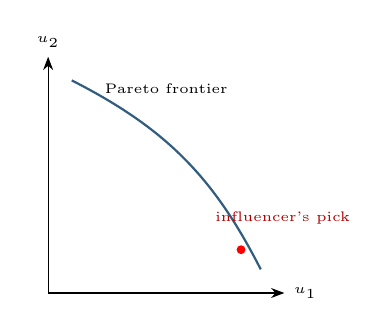
\begin{tikzpicture}[>=Stealth, font=\tiny]
	  \draw[->] (0,0)--(3,0) node[right]{$u_{1}$};
	  \draw[->] (0,0)--(0,3) node[above]{$u_{2}$};
	  \draw[blau-upc, thick] (0.3,2.7) to[bend left=18] (2.7,0.3);
	  \node at (1.5,2.6) {\tiny Pareto frontier};
	  \fill[red] (2.45,0.55) circle (1.6pt);
	  \node[right, font=\tiny, text=red!70!black] at (2.0,0.95) {influencer's pick};
	\end{tikzpicture}
	\vskip1mm
	{\tiny\itshape moves first $\Rightarrow$ grabs its favourite corner of the frontier}
	\end{center}
	\end{column}
	\end{columns}
}

\frame{\frametitle{The generalized commitment race: entanglement}
	\begin{block}{Why agents are not incentivised to make Pareto improvements}
		{\tiny
		\begin{itemize}
			\item When you choose your program in an open-source game, you optimise against your \emph{subjective distribution} over the opponent's possible programs -- including \textbf{counterfactual} ones (programs they might have submitted but didn't).
			\item So you cannot simply maximise against the opponent's \emph{actual} program: doing so might make you worse off against \emph{counterfactual} versions. Your incentive is \textbf{entangled} with those counterfactual programs.
			\item Equivalently: whenever a rational agent ``\emph{punishes}'' an opponent (for, say, proposing a Pareto improvement), it is \emph{forgoing utility against the actual program} to gain utility against some \emph{counterfactual} program.
			\item \textbf{Entanglement is the obstacle:} it is exactly what disincentivises accepting a Pareto improvement (accepting might look ``soft'' and cost you against a counterfactual hawk). This is the \emph{generalized} commitment race -- it persists even with full conditional commitment.
		\end{itemize}
		}
	\end{block}
}

%==================================================================
\section{Safe Pareto improvements}
%==================================================================

\frame{\frametitle{Safe Pareto improvements (SPI)}
	\begin{block}{Improving on a default that risks conflict}
		{\tiny
		\begin{itemize}
			\item Setup (Oesterheld--Conitzer; DiGiovanni--Clifton--Mac\'e, arXiv:2403.05103): players delegate to \emph{representative} programs. The \emph{default} instruction is ``play the original game as best you can''.
			\item An \textbf{SPI} is a re-instruction (restrict the strategy set, or re-map utilities) that is \textbf{guaranteed to make \emph{every} player weakly better off} -- with \emph{no} probabilistic assumptions about how the representatives play. A Pareto improvement that is \emph{safe} because it improves \emph{regardless} of the opponent.
			\item Example: a game heading for costly conflict (Chicken-style). Agree on a transformation that strips out the mutually destructive outcome; each player does at least as well, whatever happens.
			\item The paper proves a clean guarantee -- the \textbf{Pareto Meet Minimum (PMM)}: each player gets at least their \emph{lowest payoff over efficient (Pareto-optimal) outcomes}, and this bound is \emph{tight} (renegotiation cannot promise more). Next slide: why. Caveat: it needs a strong assumption.
		\end{itemize}
		}
	\end{block}
}

\frame{\frametitle{Why an SPI guarantees a floor: the Pareto Meet Minimum}
	\begin{columns}[T]
	\begin{column}{0.58\textwidth}
	\begin{block}{The shape of the renegotiation set controls exploitation}
		{\tiny
		\begin{itemize}
			\item Each agent's \emph{renegotiation set} is the Pareto-improvements it will accept. On the frontier, ``better for the opponent'' \emph{means} ``worse for me''.
			\item Let $A$ be the frontier point \textbf{best for me} (worst for the opponent). I have every reason to include points \emph{up to} $A$: pushing the opponent below $A$'s level cannot help me -- by definition $A$ already maximises \emph{my} payoff on the frontier.
			\item But including points \emph{beyond} $A$ (where I would accept being worse than at $A$) enables \textbf{exploitation}: the opponent could make herself better off by making me worse off.
			\item So rational renegotiation sets stop at each player's $A$-point. The worst the agreed outcome can be for me is the \emph{opponent's} $A$-point -- my \textbf{lowest efficient payoff}. That guaranteed floor is the \textbf{PMM} (and it is tight).
		\end{itemize}
		}
	\end{block}
	\end{column}
	\begin{column}{0.42\textwidth}
	\begin{center}
	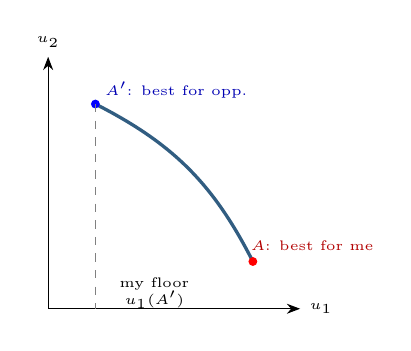
\begin{tikzpicture}[>=Stealth, font=\tiny]
	  \draw[->] (0,0)--(3.2,0) node[right]{$u_{1}$};
	  \draw[->] (0,0)--(0,3.2) node[above]{$u_{2}$};
	  \draw[blau-upc, very thick] (0.6,2.6) to[bend left=18] (2.6,0.6);
	  \fill[red] (2.6,0.6) circle (1.6pt); \node[above right,font=\tiny,text=red!70!black] at (2.45,0.62) {$A$: best for me};
	  \fill[blue] (0.6,2.6) circle (1.6pt); \node[above right,font=\tiny,text=blue!70!black] at (0.6,2.55) {$A'$: best for opp.};
	  \draw[dashed,gray] (0.6,2.6)--(0.6,0);
	  \node[font=\tiny,align=center] at (1.35,0.2) {my floor\\ $u_1(A')$};
	\end{tikzpicture}\\[1mm]
	{\tiny\itshape accept the frontier between $A'$ and $A$, never beyond}
	\end{center}
	\end{column}
	\end{columns}
}

\frame{\frametitle{The assumption SPI relies on -- and the cheating problem}
	\begin{block}{Participation independence}
		{\tiny
		\begin{itemize}
			\item \textbf{Participation independence:} representatives behave the \emph{same} in the SPI-transformed game as in the default game -- their play does not change just because an SPI is in effect. This independence is what lets you \emph{guarantee} the improvement.
			\item But it is unrealistic. \textbf{The cheating problem:} if I know that an SPI will Pareto-improve away any conflict, then conflict is \emph{less costly} for me, so I am incentivised to submit a \emph{more hawkish} default program.
			\item Anticipating my hawkishness, my opponent's incentive to offer the SPI in the first place is undermined. \textbf{The SPI can defeat itself} -- precisely the entanglement effect, reappearing.
		\end{itemize}
		}
	\end{block}
}

\frame{\frametitle{Entanglement-free SPI: the idea}
	\begin{block}{Make the improvement with an entanglement-free program}
		{\tiny
		\begin{itemize}
			\item Diagnosis: \emph{entanglement} (caring about counterfactual opponent programs) is what disincentivises Pareto improvements. So make the improvement using a separate program that is \textbf{entanglement-free} -- the \textbf{renegotiation program}.
			\item \textbf{Sequential structure:} agents \emph{first} exchange renegotiation programs and \emph{update on the actual one}; \emph{then} submit their default programs.
			\item Because you update on the opponent's \emph{actual} renegotiation program, you optimise against \emph{it}, not against counterfactual versions $\Rightarrow$ \emph{no entanglement} $\Rightarrow$ no incentive to punish/reject improvements.
			\item The renegotiation program may \emph{only propose Pareto improvements} (conditional on the opponent's default program). Two consequences:
			\begin{itemize}\scriptsize
				\item[--] it can \emph{never make the opponent worse off} $\Rightarrow$ no influencer-responder exploitation, \emph{even though} it moves first;
				\item[--] it \emph{conditions on the default program} $\Rightarrow$ it can \emph{detect} hawkish ``cheating'' defaults and withhold improvements, restoring unexploitability and \textbf{removing reliance on participation independence}.
			\end{itemize}
			\item You keep your full action space: you can still play the open-source game with your default program; the renegotiation program only \emph{adds} the option to Pareto-improve.
		\end{itemize}
		}
	\end{block}
}

\frame{\frametitle{Entanglement-free SPI: the protocol}
	\begin{columns}[T]
	\begin{column}{0.56\textwidth}
	\begin{block}{A clean formalism}
		{\tiny
		\begin{itemize}
			\item Open-source game: actions $A=A_1\times A_2$, utilities $u_i:A\to\mathbb{R}$, programs $p_i:P_{-i}\to A_i$, joint action $a=\big(p_1(p_2),\,p_2(p_1)\big)$.
			\item \textbf{Renegotiation function} $rn_i:RN_{-i}\times A\to\mathcal{C}(A)$: conditional on the opponent's renegotiation function, it proposes a \emph{set} of Pareto-improvements on the default outcome $a$. A rule $\mathrm{sel}$ picks one point of the agreed intersection.
			\item \textbf{Entanglement-free renegotiation program} $en_i:P_{-i}\to RN_i$ reads the opponent's \emph{default} program, outputs a renegotiation function.
			\item The intersection $I = rn_1(rn_2,a)\cap rn_2(rn_1,a)$ holds the Pareto-improvements \emph{both} agents will make; $\mathrm{sel}(I)$ is the final outcome. (Choosing $\mathrm{sel}$ adds no coordination problem, under mild conditions -- DiGiovanni.)
		\end{itemize}
		}
	\end{block}
	\end{column}
	\begin{column}{0.44\textwidth}
	\begin{center}
	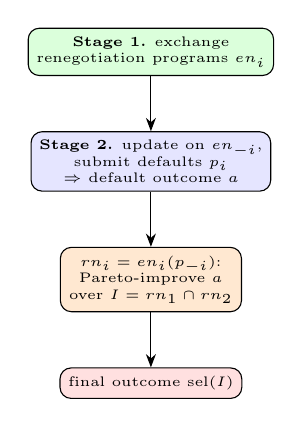
\begin{tikzpicture}[>=Stealth, font=\tiny,
	   b/.style={draw, rounded corners, align=center, inner sep=3pt, minimum width=23mm}]
	  \node[b, fill=green!14] (s1) {\textbf{Stage 1.} exchange\\ renegotiation programs $en_i$};
	  \node[b, fill=blue!10, below=7mm of s1] (s2) {\textbf{Stage 2.} update on $en_{-i}$,\\ submit defaults $p_i$\\ $\Rightarrow$ default outcome $a$};
	  \node[b, fill=orange!18, below=7mm of s2] (s3) {$rn_i=en_i(p_{-i})$:\\ Pareto-improve $a$\\ over $I=rn_1\cap rn_2$};
	  \node[b, fill=red!12, below=7mm of s3] (s4) {final outcome $\mathrm{sel}(I)$};
	  \draw[->] (s1)--(s2); \draw[->] (s2)--(s3); \draw[->] (s3)--(s4);
	\end{tikzpicture}
	\end{center}
	\end{column}
	\end{columns}
}

\frame{\frametitle{Why first-mover is safe here -- and what we trade away}
	\begin{block}{Resolving the race without creating a new one}
		{\tiny
		\begin{itemize}
			\item Usually, a sequential structure creates an influencer-responder race (the first mover grabs the frontier). Here the first move (renegotiation) can \emph{only Pareto-improve}, so it \textbf{cannot exploit} -- no new commitment race is introduced.
			\item Net result: entanglement-free SPI \textbf{solves the cheating problem} and \textbf{drops the participation-independence assumption} (the renegotiation program conditions on the defaults to catch cheating), while the sequential structure \textbf{avoids introducing its own commitment race}.
			\item \textbf{The trade-off -- no tight PMM.} The renegotiation program conditions on the default program, so it can create an \emph{incentive gradient}: ``more cooperative default $\Rightarrow$ I offer more Pareto-improvement; more hawkish $\Rightarrow$ less''. Because it may \emph{withhold} improvement to shape the opponent's default, the agreed set is no longer the full ``up-to-$A$'' set, and the tight \textbf{Pareto Meet Minimum} floor is lost. Weaker (more realistic) assumptions buy a weaker guarantee.
		\end{itemize}
		}
	\end{block}
	{\tiny \hfill (Entanglement-free SPI: Daniel C; selection-function coordination after DiGiovanni.)}
}

\end{document}
